\chapter{Conversion Service}

\section{Methodology}
As stated in 2.1, there is no standardized format for WSIs. Supplement 145 of the DICOM standard tries to unify the whole process around WSIs, but vendors still push their proprietary formats. For the reasons mentioned in 2.1.3, it is necessary to establish a common format for all the WSIs which are subject to the process chain established in 2.4. Therefore, the goal of the CS is to convert WSIs of proprietary formats into a common open format.

To make the conversion as convenient and fast as possible, the CS should only have brief user interaction. For this purpose it will not have a GUI but be done as a console script. Furthermore, it shouldn't be necessary to restart the conversion for every WSI to convert. Instead, the CS will take an input directory as parameter and convert all WSIs of a valid format inside this directory. Another parameter will be a specified output folder, in which the DZIs are stored.

\begin{table}[H]
	\begin{center}
		\begin{tabular}{| l | l |}
			\hline
			\textbf{vendor} & \textbf{formats}\\ \hline
			Aperio & SVS, TIF\\ \hline
			Hamamatsu & VMS, VMU, NDPI\\ \hline
			Leica & SCN\\ \hline
			3DHistech/Mirax & MRXS\\ \hline
			Philips & TIFF\\ \hline
			Sakura & SVSLIDE\\ \hline
			Trestle & TIF\\ \hline
			Ventana & BIF, TIF\\ \hline
		\end{tabular}
		\caption{File formats by vendor}
		\label{tab3.1}
	\end{center}
\end{table}

Tab. \ref{tab3.1} gives an overview of file formats, sorted by vendor, which are viable as input for the conversion.


\subsection{Selection of Image Format}
\begin{table}[H]
	\begin{center}
		\begin{tabular}{| p{3cm} | p{4cm} | p{2.5cm} |}
			\hline
			\textbf{tool} & \textbf{description} & \textbf{image format} \\
			\hline
			Deep Zoom Composer & dekstop app for Windows & DZI \\ \hline
			Image Composite Editor & panoramic image stitcher from Microsoft Research for the Windows desktop & DZI \\ \hline
			DeepZoomTools.dll & .NET-library, comes with Deep Zoom Composer & DZI \\ \hline
			deepzoom.py & Python & DZI \\ \hline
			deepzoom & Perl utility & DZI \\ \hline
			PHP Deep Zoom Tools & PHP & DZI \\ \hline
			Deepzoom & PHP & DZI \\ \hline
			DZT & an image slicing library and tool written in Ruby & DZI \\ \hline
			MapTiler &  desktop app for Windows, Mac, Linux & TMS \\ \hline
			VIPS & command line tool and library for a number of languages & DZI \\ \hline
			Sharp & Node.js, uses VIPS & DZI \\ \hline
			MagickSlicer & shell script (Linux/Mac) & DZI \\ \hline
			Gmap Uploader Tiler & C++ & DZI \\ \hline
			Node.js Deep Zoom Tools & Node.js, under construction & DZI \\ \hline
			OpenSeaDragon DZI Online Composer & Web app (and PERL and PHP scripts) & DZI \\ \hline
			Zoomable & service, offers embeds; no explicit API & DZI \\ \hline
			ZoomHub & service, under construction & DZI \\ \hline
			Kakadu & C++ library to encode or decode JPEG 2000 images & IIIF \\ \hline
			PyramidIO & Java (command line and library) & DZI \\ \hline
		\end{tabular}
		\caption{Overview of conversion options for zooming image formats (source: \cite{web:openseadragon})}
		\label{tab3.2}
	\end{center}
\end{table}

A format or service must be chosen as conversion target for the CS. Choices have been established in 2.1.3. These are:
\begin{enumerate}[(1)]
	\item BigTIFF
	\item DZI
	\item IFFF
	\item JPEG 2000
	\item TMS/OMS
\end{enumerate}

To convert a WSI, a conversion tool is needed. Tab. \ref{tab3.2} shows a listing of possibilities for that purpose. Listed are the name of the tool, used technology and output format. It shows clearly, that DZI has a great variety of options, while the alternatives have little to none (Map Tiler for TMS, Kakadu for IFFF and none for the others).

Since the CS should only consist of brief user interaction and be as automated as possible, desktop and web applications are not valid as tools for conversion. This excludes \emph{Deep Zoom Composer}, \emph{MapTiler}, \emph{OpenSeaDragon DZI Online Composer} and \emph{Zoomable} as possible choices (therefore also excluding, next to other reasons\footnote{compare chap 2.1.3}, TMS as possible format).

One of the reasons not to use proprietary formats was the support of only certain operating systems, eliminating Windows-only tools. Those are \emph{Image Composite Editor} and \emph{DeepZoomTools.dll}.

Furthermore, reading the proprietary formats is a highly specialized task, eliminating most of the leftover choices: \emph{deepzoom}\cite{web:deepzoom}, \emph{DZT}\cite{web:dzt}, \emph{sharp}\cite{web:sharp}, \emph{MagickSlicer}, \emph{Node.js Deep Zoom Tools}\footnote{MagickSlicer and Node.js Deep Zoom Tools use ImageMagick to read images, which doesn't support any of the proprietary WSI formats\cite{web:imagemagick}.}, \emph{Gmap Uploader Tiler}\cite{web:gmap}, Zoomhub\cite{web:zoomhub} and \emph{PyramidIO}\cite{web:pyramidio}.

\emph{Kakadu} can only encode and decode JPEG 2000 images\cite{web:openseadragon}, making it no valid choice either.

This leaves \emph{deepzoom.py} and \emph{VIPS}, both creating DZI as output.


\subsection{Deepzoom.py}

Deepzoom.py\footnote{See \url{https://github.com/openzoom/deepzoom.py} for further details} is a python script and part of Open Zoom\footnote{See \url{https://github.com/openzoom} for further details}. It can either be called directly over a terminal or imported as a module in another python script. The conversion procedure itself is analogous for both methods.

If run in a terminal the call looks like the following:

\begin{lstlisting}
	$ python deepzoom.py [options] [input file]
\end{lstlisting}

The various options and their default values can be seen in tab. 3.2. If called without a designated output destination, deepzoom.py will save the converted dzi right next to the original input file.

\begin{table}[H]
	\begin{center}
		\begin{tabular}{| r | l | r |}
			\hline
			\textbf{option} & \textbf{description} & \textbf{default} \\ \hline
			-h & show help dialog & - \\ \hline
			-d & output destination & - \\ \hline
			-s & size of the tiles in pixels & 254 \\ \hline
			-f & image format of the tiles & jpg\\ \hline
			-o & overlap of the tiles in pixels (0 - 10) & 1 \\ \hline
			-q & quality of the output image (0.0 - 1.0) & 0.8 \\ \hline
			-r & type of resize filter & antialias \\ \hline
		\end{tabular}
		\caption{Options for deepzoom.py}
	\end{center}
\end{table}

The resize filter is applied to interpolate the pixels of the image when changing its size for the different levels. Supported filters are:

\begin{itemize}
	\item cubic
	\item biliniear
	\item bicubic
	\item nearest
	\item antialias
\end{itemize}

When used as module in another python script, deepzoom.py can simply be imported via the usual \emph{import} command. To actually use deepzoom.py, a Deep Zoom Image Creator needs to be created. This class will manage the conversion process:

\begin{lstlisting}[frame=single]
# Create Deep Zoom Image Creator
creator = deepzoom.ImageCreator(tile_size=[size], 
	tile_overlap=[overlap],	tile_format=[format], 
	image_quality=[quality], resize_filter=[filter])
\end{lstlisting}

The options are analogous with the terminal version (compare tab. 3.2). To start the conversion process, the following call must be made within the python script:

\begin{lstlisting}[frame=single]
# Create Deep Zoom image pyramid from source
creator.create([source], [destination])
\end{lstlisting}

Upon calling, the ImageCreator opens the input image $img_{input}$ and creates a description with all the needed information for the dzis describing xml file\footnote{Compare chap. 2.1.1}. After that, the number of levels is calculated. For this, the bigger value of height and width of $img_{input}$ is chosen (see eq. 3.1) and then used to determine the number of levels $lvl$ (see eq. 3.2).

\begin{equation}
	max{\_}dim = max(height, width)
\end{equation}

\begin{equation}
	lvl = {\lceil}log_2(max{\_}dim) + 1\rceil
\end{equation}

Once $lvl$ has been determined, $img_{input}$ will be resized in the chosen quality (-q/image{\textunderscore}quality) for every level $i$, with $i \in (0, lvl-1)$. The new resolution will be calculated for both dimensions $dim$ with a function $scale$ (see eq. 3.3) analogously. Furthermore, the image will be interpolated with the specified filter (-r/resize{\textunderscore}filter). The resized image will be called $img_i$.

\begin{equation}
	scale = {\lceil}dim * 0.5^{lvl-i}\rceil
\end{equation}

Once $img_i$ has been created, it will be tessellated into as many tiles of the specified size (-s/tile{\textunderscore}size) and with the specified overlap (-o/tile{\textunderscore}overlap) as possible. Since not every image will be of the size $2^n, n \in $ in either dimension, it is highly likely that the set of tiles for the last column/row will be smaller then specified in either dimension.

Every tile will be saved as [column]{\textunderscore}[row].[format] ([format] depending on -f/file{\textunderscore}format) in a folder called according to the corresponding level $i$. This folder will be located inside another folder, called [filename]{\textunderscore}files. The describing xml file will be persisted as [filename].dzi on the same level.


\subsection{VIPS}

VIPS (VASARI Image Processing System)\nmc{VIPS}{VASARI Image Processing System} describes itself as "[...] a free image processing system [...]" \cite{web:vips}. It includes a wide range of different image processing tools, such as various filters, histograms, geometric transformations and color processing algorithms. It also supports various scientific image formats, especially those needed for the Conversion Service\footnote{See chap. 2.2.1}\cite{web:vips}.

VIPS comes in two parts: the actual library (called libvips) and a GUI (called nip2). libvips offers interfaces for C, C++, python and the command line. The GUI will not be further discussed, since it is of no interest for the implementation of the Conversion Service.

One of the strongest traits of VIPS is its speed and little data usage compared to other imaging libraries\cite{cupitt05}. Given the task of the Conversion Service to convert WSIs of various formats, which tend to be quite large, both of those perks are especially welcome.

VIPS superior speed and little data usage comes from a fully demand-driven image input/output system. While conventional imaging libraries queue their operations and go through them sequentially, VIPS awaits a final write command, before actually manipulating the image. All the queued operations will then be evaluated and molded into a few single operations. Thus, requiring no additional disc space for intermediates and no unnecessary disc in- and output. Furthermore, if more than one CPU is available, VIPS will automatically evaluate in parallel\cite{cupitt96}.

As mentioned before, VIPS has a command line and python interface. In either case, a function called \emph{dzsave(...)} will manage the conversion from a WSI to a dzi. A call in the terminal will look like the following:

\begin{lstlisting}
$ vips dzsave [input] [output] [options]
\end{lstlisting}

When called, VIPS will take the image [input], convert it into the dzi file format and then save it to [output]. The various options and their default values can be seen in tab. 3.3. 

\begin{table}[H]
	\begin{center}
		\begin{tabular}{| l | l | l |}
			\hline
			\textbf{option} & \textbf{description} & \textbf{default} \\ \hline
			layout & directory layout (allowed: dz, google, zoomify) & dz \\ \hline
			overlap & tile overlap in pixels & 1 \\ \hline
			centre & center image in tile & false \\ \hline
			depth & pyramid depth & onepixel \\ \hline
			angle & rotate image during save & d0 \\ \hline
			container & pyramid container type & fs \\ \hline
			properties & write a properties file to the output directory & false \\ \hline
			strip & strip all metadata from image & false \\ \hline
		\end{tabular}
		\caption{Options for VIPS}
	\end{center}
\end{table}

A call in python does have the same parameters and default values. It looks like this:

\begin{lstlisting}[frame=single]
image = Vips.Image.new_from_file(input)
image.dzsave(output[, options])
\end{lstlisting}

In line 1 the image gets opened and saved into \emph{image}. While being opened, further operations could be done. The command in line 2 writes the processed image into the specified output location.


\section{Implementation}

As stated before, the Conversion Service is implemented as a python script. The first iteration of the script used deepzoom.py for the conversion. This caused severe performance issues though. Out of all the image files in the test set\footnote{See chap. 3.3}, only one could be converted\footnote{CMU-3.svs from Aperio, see Appendix A}. Every other file was either too big, so the process would eventually be killed by the operating system or exit with an IOError concerning the input file from the PIL imaging library. The second iteration of the Conversion Service uses VIPS, which is faster then deepzoom.py and also capable of converting all the given test images.

The script has to be called inside a terminal in the following fashion:

\begin{lstlisting}
	$ python ConversionService.py [input dir] [output dir]
\end{lstlisting}

It is mandatory to specify the input and output directory in the call, so the script knows where to look for images up to conversion and where to save the resulting dzi files.

Upon calling, the \emph{main()} routine will be started, which orchestrates the whole conversion process. It looks as follows:

\begin{lstlisting}[frame=single]
def main():
	path = checkParams()
	files = os.listdir(path)
	for file in files:
		print("-----------------------------------------")
		extLen = getFileExt(file)
		if(extLen != 0):
			print("converting " + file + "...")
			convert(path, file, extLen)
			print("done!")
\end{lstlisting}

\emph{checkParams()} checks if the input parameters are valid and, if so, returns the path to the specified folder or exit otherwise. Furthermore, it will create the specified output folder, if it doesn't exist already. In the next step, the specified input folder will be checked for its content. \emph{getFileExt(file)} looks up the extension of each contained file and will either return the length of the files extension or $0$ otherwise. Each valid file will then be converted with the \emph{convert(...)} function:

\begin{lstlisting}[frame=single]
# convert image source into .dzi format
# param path: directory of param file
# param file: file to be converted
# param extLen: length of file extension
def convert(path, file, extLen):
	dzi = OUTPUT + file[:extLen] + "dzi"
	im = Vips.Image.new_from_file(path + file)
	im.dzsave(dzi, overlap=OVERLAP, tile_size=TILESIZE)
\end{lstlisting}

The name for the new dzi file will be created from the original file name, however, the former extension will be replaced by "dzi" (see line 6). \emph{OUTPUT} specifies the output directory which the file will be saved to. Next, the image file will be opened with Vips' Image class. Afterwards, \emph{dzsave(...)} will be called, which handles the actual conversion into the dzi file format. \emph{OVERLAP} and \emph{TILESIZE} are global variables which describe the overlap of the tiles and their respective size. Their values are 0 (\emph{OVERLAP}) and 256 (\emph{TILESIZE}). The output will be saved to the same folder as ConversionService.py is operating from, plus "/dzi/[\emph{OUTPUT}]/".


\section{Test}

To test the correct functionality of the Conversion Service, test data is needed. OpenSlide offers a selection of freely distributable data\footnote{See OpenSlides Homepage: \url{http://openslide.cs.cmu.edu}, or directly for the test data: \url{http://openslide.cs.cmu.edu/download/openslide-testdata/}}, which can be used for that purpose.

Since the WSIs are of enormous size, they are not delivered via the repository. Instead they need to be downloaded separately from the OpenSlide homepage. For a complete listing of the used test data see Appendix A.


\subsection{Setup}

To create a controlled environment for the test, a new directory will be created, called \emph{CS{\textunderscore}test}. A copy of ConversionService.py as well as a directory containing all the test WSIs (called \emph{input}) will be placed in that directory.

\emph{Input} contains the following slides:

\begin{enumerate}[(1)]
	\item CMU-2 (Aperio, .svs)
	\item CMU-1 (Generic Tiled tiff, .tiff)
	\item OS-3 (Hamamatsu, .ndpi)
	\item CMU-2 (Hamamatsu, .vms)
	\item Leica-2 (Leica, .scn)
	\item Mirax2.2-3 (Mirax, .mrxs)
	\item CMU-2 (Trestle, .tif)
	\item OS-2 (Ventana, .bif)
\end{enumerate}

Because of their structure, (4), (6) and (7) will be placed in directories titled with their file extension. Fig. 3.2 shows the content of the input folder.

\begin{figure}[H]
	\begin{center}
		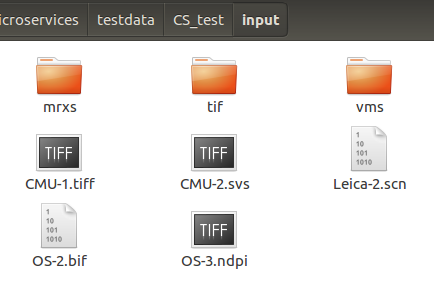
\includegraphics[scale=0.5]{img/inputDir.png}
		\caption{Content of input directory}
		\label{fig:fig3.2}
	\end{center}
\end{figure}

This makes multiple calls of the Conversion Service necessary. The calls, in that order, are:

\begin{lstlisting}
	$ python ConversionService.py input/ out_1/
	$ python ConversionService.py input/mrxs out_2/
	$ python ConversionService.py input/tif out_3/
	$ python ConversionService.py input/vms out_4/
\end{lstlisting}


\subsection{Result}

All runs of ConversionService.py were successful. Tab. 3.3 shows an overview of the results:

\begin{table}[H]
	\begin{center}
		\begin{tabular}{| l | l | r |}
			\hline
			\textbf{input} & \textbf{output} & \textbf{time (sec)} \\ \hline
			input/ & CMU-1.dzi, CMU-2.dzi, Leica-2.dzi, OS-2.dzi, OS-3.dzi & 1992 \\ \hline
			input/mrxs/ & Mirax2.2-3.dzi & 500 \\ \hline
			input/tif/ & CMU-2.dzi & 56 \\ \hline
			input/vms/ & CMU-2-40x - 2010-01-12 13.38.58.dzi & 305 \\ \hline
		\end{tabular}
		\caption{Results of Conversion Service Test}
	\end{center}
\end{table}

The vast difference in file size of the test data accounts for the different run times of the tests. While the first test converted 5 WSIs (399 sec/WSI), every other test converted a single one. The conversion of (6) was much faster, since the file was smaller in size (304.22 MB) compared to the others (1495.24 MB on average).